\subsection{PlayerList}
PlayerList er en klasse der holder styr på spillets spillere. PlayerList har en metode "PlayerList" som ud fra et givent antal spillere, opretter spillerne i et array og tildeler dem navn, farve, konto og nummer. Denne metode benyttes i GameController klassens metode gameSetup.
\begin{figure}[H]
    \centering
    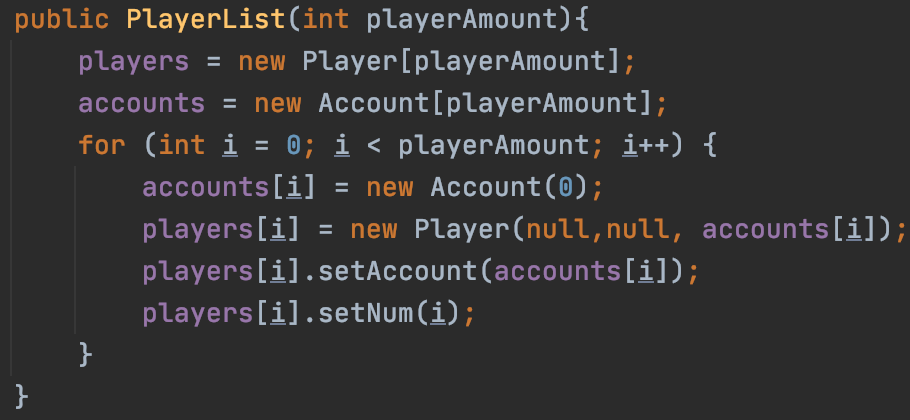
\includegraphics[width=\textwidth]{sources/7_implementering/PlayerList PlayerList.png}
    \caption{PlayerList metoden i PlayerList klassen}
    \label{fig:readFile}
\end{figure}



\subsubsection{Player}
Player klassen er ansvarlig for at definere de attributter som en spiller skal have. Spilleren skal have både navn, farve, briktype, konto og et nummer. Player klassen har også metoden "move", som ud fra spillerens position, et ønsket antal felter og listen med felter, kan rykke spilleren. Samtidig har player klassen en boolean værdi som afgør om spilleren er placeret i fængsel eller ej.
\begin{figure}[H]
    \centering
    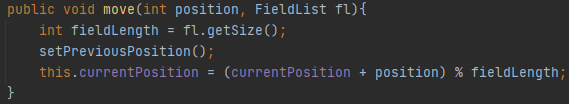
\includegraphics[width=\textwidth]{sources/7_implementering/move-method.png}
    \caption{move metoden i Player klassen}
    \label{fig:readFile}
\end{figure}

\subsubsection{Account}
Account klassen har en enkelt attribut; balance. Balance er kontoens pengebeholdning og der er hertil metoder hvormed man kan trække penge eller indbetale penge ved navn "withdraw" og "deposit".